\newcommand{\nodeLabel}[3]{
    \node[color=#3, fill=white, opacity=0.9] at (#1) {\fontsize{10}{10}\selectfont #2}
}

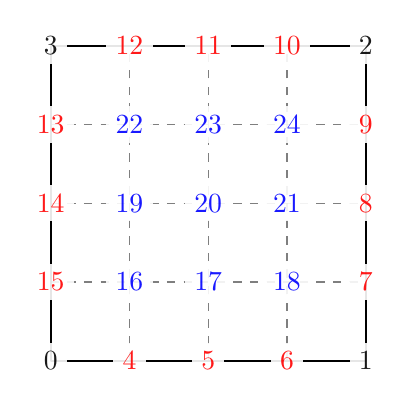
\begin{tikzpicture}[line join=bevel,scale=2,>=latex]
  \coordinate (n0) at (-1,-1);
  \coordinate (n1) at (1,-1);
  \coordinate (n2) at (1,1);
  \coordinate (n3) at (-1,1);

  \coordinate (n4) at (-0.5, -1);
  \coordinate (n5) at (0, -1);
  \coordinate (n6) at (0.5, -1);

  \coordinate (n7) at (1, -0.5);
  \coordinate (n8) at (1, 0);
  \coordinate (n9) at (1, 0.5);

  \coordinate (n10) at (0.5, 1);
  \coordinate (n11) at (0, 1);
  \coordinate (n12) at (-0.5, 1);

  \coordinate (n13) at (-1, 0.5);
  \coordinate (n14) at (-1, 0);
  \coordinate (n15) at (-1, -0.5);

  \coordinate (n16) at (-0.5, -0.5);
  \coordinate (n17) at (0, -0.5);
  \coordinate (n18) at (0.5, -0.5);

  \coordinate (n19) at (-0.5, 0);
  \coordinate (n20) at (0, 0);
  \coordinate (n21) at (0.5, 0);

  \coordinate (n22) at (-0.5, 0.5);
  \coordinate (n23) at (0, 0.5);
  \coordinate (n24) at (0.5, 0.5);
  
  
  \draw[thick] (n0) -- (n1) -- (n2) -- (n3) -- cycle;
  \draw[dashed,opacity=0.5] (n4) -- (n12);
  \draw[dashed,opacity=0.5] (n5) -- (n11);
  \draw[dashed,opacity=0.5] (n6) -- (n10);
  \draw[dashed,opacity=0.5] (n15) -- (n7);
  \draw[dashed,opacity=0.5] (n14) -- (n8);
  \draw[dashed,opacity=0.5] (n13) -- (n9);

  \nodeLabel{n0}{0}{black};
  \nodeLabel{n1}{1 }{black};
  \nodeLabel{n2}{2 }{black};
  \nodeLabel{n3}{3 }{black};
  \nodeLabel{n4}{4 }{red};
  \nodeLabel{n5}{5 }{red};
  \nodeLabel{n6}{6 }{red};
  \nodeLabel{n7}{7 }{red};
  \nodeLabel{n8}{8 }{red};
  \nodeLabel{n9}{9 }{red};
  \nodeLabel{n10}{10}{red};
  \nodeLabel{n11}{11}{red};
  \nodeLabel{n12}{12}{red};
  \nodeLabel{n13}{13}{red};
  \nodeLabel{n14}{14}{red};
  \nodeLabel{n15}{15}{red};
  
  \nodeLabel{n16}{16}{blue};
  \nodeLabel{n17}{17}{blue};
  \nodeLabel{n18}{18}{blue};
  \nodeLabel{n19}{19}{blue};
  \nodeLabel{n20}{20}{blue};
  \nodeLabel{n21}{21}{blue};
  \nodeLabel{n22}{22}{blue};
  \nodeLabel{n23}{23}{blue};
  \nodeLabel{n24}{24}{blue};

\end{tikzpicture}